%%%%%%%%%%%%%%%%%%%%%%%%%%%%%%%%%%%%%%%%%%%%%%%%%%%%%%%
%%                SBD scalable design                %%
%%%%%%%%%%%%%%%%%%%%%%%%%%%%%%%%%%%%%%%%%%%%%%%%%%%%%%%
\chapter{Scalable set based design optimization}
\chaptermark{Scalable set based design optimization}
\label{ch:scalableSBD}
%%%%%%%%%%%%%%%%%%%%%%%%%%%%%%%%%%%%%%%%%%%%%%%%%%%%%%%

This chapter describes a novel design tool for identifying a set of scalable designs for product remanufacturing using parametric design optimization. Scalability is an enabler for product remanufacturing since it provides components with the flexibility to have their specifications upgraded to meet higher requirement levels.

The methodology in this chapter is demonstrated using an industrial case study for the remanufacturing of a \ac{TRS}. The thermomechanical model described in Section~\ref{sec:thermomech} along with the load case in Section~\ref{subsec:iploadcase} is used to define the design variables and uncertain parameters involved in the remanufacturing design problem. Remanufacturing is performed by \ac{AM} using laser \ac{DED}. However, our methodology can be extended to remanufacturing problems where subtractive manufacturing is used.

We begin by defining the methodology for obtaining the set-based solutions for arbitrary design and parameters spaces in Section~\ref{sec:SBDmethods}. We then demonstrate the methodology for the remanufacturing of the \ac{TRS} in Section~\ref{sec:SBDusecase}. We provide some insights and conclusions about the uses and limitations of the developed framework in Section~\ref{sec:scalableSBDsummary}.

%============================ METHODOLOGY ============================%
\section{Methodology} \label{sec:SBDmethods}

Engineering design optimization problems involve decision variables $\mathbf{x}  \in \mathbb{R}^n$ and design parameters ${\mathbf{p}}  \in \mathbb{R}^m$. Objective (${f}(\mathbf{x};\mathbf{p})$) and constraint ($\mathbf{g}(\mathbf{x};\mathbf{p})$) functions are used to reflect design requirements. Given bounded design optimization variables and parameters $\mathbf{L} \leq \mathbf{x} \leq \mathbf{U}$ and $\mathbf{L}_p \leq \mathbf{p} \leq \mathbf{U}_p$, respectively, we define the design space $\mathit{D}$ and the parameters space $\mathit{P}$. We also consider constraint sets $\mathit{C}_u$ for $u = 1,2,\ldots,q$ where $q$ is the number of constraints. In a product design context, constraints are part of the design requirements and are driven by the parameters $\mathbf{p}$. Finally, the feasible set $\mathit{F}$ is defined as the intersection of all constraint sets and contains designs that meet all design requirements. The set $\mathit{F}$ is the \ac{FDS} and represents the outcome of \ac{SBD} before elimination of potential designs. 

Design parameters may affect the optimal solution of the optimization problem due to their influence on design requirements. As a result, designs that are optimal throughout the parameters space $\mathit{P}$ and satisfy the design requirements comprise the set of parametric optimal designs which is a reduction of the \ac{FDS}. Since practical \ac{SBD} methodolog\-ies require solutions sets that can be easily communicated across design teams, response surfaces are used as a surrogate model to evaluate feasibility and performance and to classify membership of each design to the feasible set and the set of parametric optimal designs. 

% --------------------------- Surrogate modeling ------------------------------ %
\subsection{Surrogate modeling} \label{subsec:RSM}

The objective and constraint functions used to represent design requirements are evaluated using computer-aided engineering (CAE) tools that model the repair/remanufacturing process.  
These computational models are computationally expensive. Any SBD methodology requires a large number of function evaluations to investigate not only the design but also the parameters space. Therefore, we resort to building less expensive response surfaces to be used as surrogate models.

We conduct designs of experiments to sample the aggregate design and parameters spaces and then exercise the computational models at these sample points to generate adequate training data. An ensemble of surrogate models is then constructed and denoted by $\hat{f}(\mathbf{x};{\mathbf{p}})$ and $\hat{\mathbf{g}}(\mathbf{x};{\mathbf{p}})$. An open source surrogate model library is used to build the surrogates \cite{Talgorn2018,Lophaven2002}.

An order-based metric is used to assess the predictive capability of the surrogates \cite{Audet2018}. This metric ensures the consistency between the computationally expensive and surrogate model predictions. The order-based metric is also used for constructing response surfaces of the parametric optimal solutions with respect to varying design parameters in subsequent sections and is discussed using a numerical example in Section~\ref{subsec:numex}.
% is a measure of how well the ordering of function values throughout the analysis model agrees with that of the \ac{SM}. If this condition is observed in the response surface \ac{SM}, the solution to the minimization problem of the analysis model $f(\mathbf{x})$ and the surrogate model $\hat{f}(\mathbf{x})$ should be consistent. The conditions can be stated as follows and are adopted from \cite{Audet2018}:
%
%\begin{gather}
%	f(\mathbf{x}) \leq f(\mathbf{x}') \Leftrightarrow \hat{f}(\mathbf{x}) \leq \hat{f}(\mathbf{x}'),~\textrm{for all}~\mathbf{x}, \mathbf{x'} \in \mathit{D} \label{eq:oeobjective}\\
%	g_u(\mathbf{x}) \leq 0 \Leftrightarrow \hat{g_u}(\mathbf{x}) \leq 0,~\textrm{for all}~\mathbf{x}, \in \mathit{D}\label{eq:oeconstraints}
%\end{gather}
%
%The frequency of violation of these rules is an indicator of the surrogate model's deficiency in capturing the global minima of its corresponding analysis model. It should also be noted that any insensitive parameters or variables should be eliminated from the analysis to alleviate the computational effort of obtaining an efficient surrogate model for optimization in terms of the \ac{OE} criterion. This elimination is demonstrated at the end of Section~\ref{subsec:thermomech}.

% --------------------------- Design space reduction based on optimization ------------------------------ %
\subsection{Parametric optimal designs} \label{subsec:SBDparametric}

We use numerical optimization to provide a set of design solutions that can address  a range of requirements. Specifically, we solve the optimization problem for different parameter values. This can be seen as a form of \ac{POA} that provides the sensitivity of optimal design variable values with respect to varying parameter values \cite{Sobieszczanski-Sobieski1982}.

The surrogate optimization problem is formulated as
\begin{equation}
	\begin{aligned}
		& \underset{\mathbf{x}}{\text{minimize}}
		& & \hat{f}(\mathbf{x};{\mathbf{p}})\\
		& \text{subject to}
		& & \hat{\mathbf{g}}(\mathbf{x};{\mathbf{p}}) \le \mathbf{0}
	\end{aligned}
	\label{eq:SBDoptproblem}
\end{equation}
and solved to obtain the solution $\mathbf{x}^*({\mathbf{p}})$. Given intervals for the parameters $\mathbf{p}$, sampling techniques can be used to obtain a set of $m$ combinations. Here, we use \ac{LH} sampling which produces a uniform random distribution over the parameters space \cite{McKay1979}
\begin{equation}
	 {\mathbf{P}} = \begin{bmatrix}
	 	\mathbf{p}_{1}^{\text T} \\ 
	 	\mathbf{p}_{2}^{\text T} \\ 
	 	\vdots \\ 
	 	\mathbf{p}_{w}^{\text T}
	\end{bmatrix} = \begin{bmatrix}
	 	p_{11} & p_{12} & \cdots & p_{1m}\\ 
	 	p_{21} & p_{22} & \cdots & p_{2m}\\ 
	 	\vdots & \vdots & \ddots & \vdots\\ 
	 	p_{w1} & p_{w2} & \cdots & p_{wm}
	\end{bmatrix}.
\end{equation}

\ac{LH} sampling is used since the number of samples needed to fit an adequate response surface scales better with dimensionality relative to uniform sampling techniques such as full factorial sampling. Once we have obtained a solution $\mathbf{x}^*({\mathbf{p}})$ for each of the $w$ parameter vectors, a response surface $\hat{\mathbf{x}^*}(\mathbf{p})$ is built using the set of parametric optimal designs $\mathbf{X}^*=  \{ \mathbf{x}^*(\mathbf{p}_1),\mathbf{x}^*(\mathbf{p}_2),\ldots,\mathbf{x}^*(\mathbf{p}_w) \}$. A rule of thumb indicates that the initial sample size should be about an order of magnitude larger than the dimensionality of the problem, i.e., $w \approx 10m$) \cite{Loeppky2008}. To potentially save computational cost, we also monitor the convergence rate of the order-based error as more samples are added and accept the response surface as adequate once it has reached an appropriate threshold. An example of this procedure is provided in Section~\ref{subsec:numex}. The response surface $\hat{\mathbf{x}^*}(\mathbf{p)}$ is used to predict parametric optimal designs throughout the parameters space.

Sensitivity gradients of the design variables with respect to the parameters allow designers to understand the effect of requirement changes to optimal designs.
The Jacobian of $\hat{\mathbf{x}^*}(\mathbf{p})$ is
\begin{equation}
	\mathbf{J}(\mathbf{p}) = \nabla\hat{\mathbf{x}^*}(\mathbf{p)} = \begin{bmatrix}
	 	\nabla\hat{x_1^*}^{\text T}(\mathbf{p}) \\ 
	 	\nabla\hat{x_2^*}^{\text T}(\mathbf{p}) \\ 
	 	\vdots \\ 
	 	\nabla\hat{x_n^*}^{\text T}(\mathbf{p})
	\end{bmatrix} = \begin{bmatrix}
	 	\frac{\partial \hat{x_1^*}}{\partial p_1} & \frac{\partial \hat{x_1^*}}{\partial p_2} & \cdots & \frac{\partial \hat{x_1^*}}{\partial p_m}\\ 
	 	\frac{\partial \hat{x_2^*}}{\partial p_1} & \frac{\partial \hat{x_2^*}}{\partial p_2} & \cdots & \frac{\partial \hat{x_2^*}}{\partial p_m}\\ 
	 	\vdots & \vdots & \ddots & \vdots\\ 
	 	\frac{\partial \hat{x_n^*}}{\partial p_1} & \frac{\partial \hat{x_n^*}}{\partial p_2} & \cdots & \frac{\partial \hat{x_n^*}}{\partial p_m}\\ 
	\end{bmatrix}.
	 \label{eq:jacobian}
\end{equation}
It can be estimated using the derivatives of the basis functions used to construct the response surface. Differentiation of the response surface is possible because it is based on a linear combination of basis functions. We use a \acf{KS} model to build  $\hat{\mathbf{x}^*}(\mathbf{p})$ and estimate the Jacobian $\mathbf{J}(\mathbf{p})$ using the linear combination of the gradient of the kernel functions. \ac{KS} was used to construct the response surface due to their immediate computation since it does not require matrix inversions. Furthermore, \ac{KS} models typically respect the order of the output which reflects its ability to predict the correct order of values of any two evaluation points. This is very important for this application since it relies on differentiating the KS model \cite{Audet2018}.

For the remainder of this subsection, let us use the typical notation between an independent variable $x$ and a dependent variable $y$ recalling however, that in our context $\hat{\mathbf{x}^*}(\mathbf{p})$ is corresponding to $y$ (dependent variable) while $\mathbf{p}$ is corresponding to $x$ (independent variable).

\ac{KS} models consist of a weighted sum of training points where the weight for each training point decreases as the distance from the prediction point increases.
\begin{multline}
 \label{eq:ksexpansion}
	\hat{y}(\mathbf{x}) = \dfrac{\sum_{j=1}^{w} \phi_j(\mathbf{x})y_j}{\sum_{j=1}^{k} \phi_j(\mathbf{x})} =
	\dfrac{\phi_1(\mathbf{x}) y_1 + \phi_2(\mathbf{x}) y_2 +\cdots + \phi_w(\mathbf{x}) y_w}{\phi_1(\mathbf{x})+ \phi_2(\mathbf{x})+\cdots + \phi_w(\mathbf{x})} = \\
	\dfrac{\phi_1(\mathbf{x}) y_1}{\phi_1(\mathbf{x})+ \phi_2(\mathbf{x}) + \cdots + \phi_w(\mathbf{x})} + \dfrac{\phi_2(\mathbf{x}) y_2}{\phi_1(\mathbf{x})+ \phi_2(\mathbf{x})+\cdots + \phi_w(\mathbf{x})} + \\
	 \cdots + \dfrac{\phi_w(\mathbf{x}) y_w}{\phi_1(\mathbf{x})+ \phi_2(\mathbf{x})+\cdots + \phi_w(\mathbf{x})},
\end{multline}
where $\phi_j$ is the kernel function for the $j$th training point, $y_j$ is the output at the $j$th training point, and $\mathbf{x}$ is the prediction point. 
%
To determine the gradient of $\hat{y}(\mathbf{x})$, the quotient rule of differentiation is applied to each term in Equation~(\ref{eq:ksexpansion}) and the common terms are factored out to yield
%\begin{table*}[h!]
%\centering
%\end{table*}
\begin{multline}
\label{eq:jacobiancomponent}
\nabla\hat{y}(\mathbf{x}) = \dfrac{\phi_1(\mathbf{x})+ \phi_2(\mathbf{x})+\cdots + \phi_w(\mathbf{x})}{\left[\phi_1(\mathbf{x})+ \phi_2(\mathbf{x})+\cdots + \phi_w(\mathbf{x})\right]^2} \times
\left[\nabla\phi_1(\mathbf{x}) y_1 + \nabla\phi_2(\mathbf{x}) y_2 +\cdots + \nabla\phi_w(\mathbf{x}) y_w\right] - \\
\dfrac{\nabla\phi_1(\mathbf{x})+ \nabla\phi_2(\mathbf{x})+ \cdots + \nabla\phi_w(\mathbf{x})}{\left[\phi_1(\mathbf{x})+ \phi_2(\mathbf{x})+\cdots + \phi_w(\mathbf{x})\right]^2} \times
\left[\phi_1(\mathbf{x}) y_1 + \phi_2(\mathbf{x}) y_2 +\cdots + \phi_w(\mathbf{x}) y_w\right] =\\
%\end{multline}
%Compacting the terms yields
%\begin{multline}
%	\label{eq:jacobiancomponent}
%	\nabla\hat{y}(\mathbf{x}) = \\
	\dfrac{{\sum_{j=1}^{w} \phi_j(\mathbf{x})} {\sum_{j=1}^{w} \nabla\phi_j(\mathbf{x})y_j}~-~{{\sum_{j=1}^{w} \nabla\phi_j(\mathbf{x})}{\sum_{j=1}^{w} \phi_j(\mathbf{x})y_j}}}{\left[\sum_{j=1}^{w} \phi_j(\mathbf{x})\right]^2}.
\end{multline}

We used the Gaussian kernel function (and its gradient ) defined as
\begin{gather}
	\label{eq:kernelfunction}
	\phi_j(\mathbf{x}) = e^{-\pi\lambda \norm{\mathbf{x}-\mathbf{x}_j}}\\
	\label{eq:kernelfunctiongrad}
	\nabla\phi_j(\mathbf{x}) = -\dfrac{\pi\lambda\left(\mathbf{x} - \mathbf{x}_j\right)}{\norm{\mathbf{x} - \mathbf{x}_j}}e^{-\pi\lambda \norm{\mathbf{x}-\mathbf{x}_j}},
\end{gather}
where $\lambda$ is the bandwidth of the kernel function. The bandwidth parameter's effect on the order-based error is also used to determine the optimal bandwidth for adequately capturing the Jacobian of the \ac{KS} model.

Equations~(\ref{eq:kernelfunction}) and (\ref{eq:kernelfunctiongrad}) are substituted into Equation~(\ref{eq:jacobiancomponent}) to provide the gradient of the prediction function $\hat{y}(\mathbf{x})$. This process is repeated for each of the design variables $\hat{x_1^*}(\mathbf{p}), \hat{x_2^*}(\mathbf{p}), \cdots \hat{x_n^*}(\mathbf{p})$ to populate the Jacobian in Equation~(\ref{eq:jacobian}). The Jacobian is used to formulate a transition rule in the parameters space to obtain the set of scalable optimal designs.

Algorithm~\ref{algo:PODalgo} presents the methodology followed to obtain the set of parametric optimal designs. The procedure including the calculation of the order-based error is demonstrated by means of a numerical example in Section~\ref{subsec:numex}.

\begin{algorithm}
	\DontPrintSemicolon % Some LaTeX compilers require you to use \dontprintsemicolon instead
	\KwIn{
		Design space bounds $\mathbf{L}$ and $\mathbf{U}$, Parameters space bounds $\mathbf{L}_p$ and $\mathbf{U}_p$, Surrogate model $\hat{f}(\mathbf{x};{\mathbf{p}})$ and $\hat{\mathbf{g}}(\mathbf{x};{\mathbf{p}})$, \ac{LH} samples of parameters space $\left[\mathbf{p}_{1},\mathbf{p}_{2}, \cdots, \mathbf{p}_{w}\right]^{\text T}$, number of cross-validation samples $n_{cv}$, \ac{LH} cross-validation set $\mathbf{X_{cv}}^*=  \{ \mathbf{x}^*(\mathbf{p}_1),\mathbf{x}^*(\mathbf{p}_2),\ldots,\mathbf{x}^*(\mathbf{p}_{n_{cv}}) \}$
	}
	\KwOut{$\mathbf{X}^*$, $\hat{\mathbf{x}^*}(\mathbf{p})$, $\nabla\hat{\mathbf{x}^*}(\mathbf{p})$}
	\For{$k \gets 1$ to $w$} {
		%				Populate possible points using LH and store them in $S_k$\;
		%				Update the RAM using built SM\;
		Solve the parametric optimization problem in Equation~(\ref{eq:SBDoptproblem}) to obtain $\mathbf{x}^*(\mathbf{p}_k)$\;
		Augment $\mathbf{X}^* \gets \mathbf{X}^* \cup \{ \mathbf{x}^*(\mathbf{p}_k) \} $\;
		Train response surface $\hat{\mathbf{x}^*}(\mathbf{p})$ using $\mathbf{X}^*$\;
		Compute order-based error up to and including $k$th sample $\varepsilon_{OE}$ using Equation~(\ref{eq:oeobjective}), $\hat{\mathbf{x}^*}(\mathbf{p})$, and $\mathbf{X_{cv}}^*$\;
	}
	Find index $k_{\textrm{min}}$ that minimizes order-based error $\varepsilon_{OE}$\;
	Set $k \gets k_{\textrm{min}} $ \;
	Set $\mathbf{X}^* \gets \mathbf{X}^*= \{ \mathbf{x}^*(\mathbf{p}_1),\mathbf{x}^*(\mathbf{p}_2),\ldots,\mathbf{x}^*(\mathbf{p}_k) \} $ \;
	Train response surface $\hat{\mathbf{x}^*}(\mathbf{p})$ using $\mathbf{X}^*$ \;
	Find bandwidth $\lambda$ that minimizes order-based error of response surface $\hat{\mathbf{x}^*}(\mathbf{p})$\;
	Compute Jacobian of response surface $\nabla\hat{{x}^*}(\mathbf{p)}$ using Equation~(\ref{eq:jacobiancomponent})\;
	\caption{Pseudo-algorithm for obtaining the set of parametric optimal designs $\mathbf{X}^*$ and \ac{KS} response surface of parameters space $\hat{{x}^*}(\mathbf{p})$}
	\label{algo:PODalgo}
\end{algorithm}

% --------------------------- Set-based design rules for AM ------------------------------ %
\subsection{Reduction to set of scalable optimal designs} \label{subsec:SBDfAM}

We adopt the terminology used by Ross et al. \cite{Ross2008} for defining the aspects of design {changeability}. 
Varying design parameters as proxies of requirements is a \textit{change agent} that provides motivation for changing the design. {Scalability} represents the ability of the design to adapt to changing requirements by means of scaling. For example, a design that is in service must now sustain a higher static load than originally intended during the design phase. This change can be accommodated by reinforcing the structure using \ac{AM} techniques. Transition rules may govern changes. For example, the reinforcement can only add material to the design and not subtract from it (analogous to the containment rule formulated by Liu and Ma \cite{Liu2017} for subtractive remanufacturing). Furthermore, there is a cost and time associated with the change. As a result, designs that minimize the transition costs while maximizing the offered alternatives should be considered during \ac{SBD} to add more value to the design. We focus here on \textit{transition rules} that consider the ability of the manufacturing process to scale the design.

We derive transition rules pertaining to additive and subtractive manufacturing. \ac{AM} processes can only add material to the substrate which results in an increase in the volume of the deposit. The opposite applies to subtractive manufacturing. The volume of the deposited part must be described in terms of the design variables pertaining to the geometry. The \textit{monotonicity} of the volume with respect to each design variable is the basis for selecting designs that are scalable. For example, a variable such as the thickness of a beam has a positive monotonicity with respect to the beam volume. This is because an increase in the beam thickness leads to an increase in beam volume. Conversely, a variable such as hole diameter through the thickness of the beam has a negative monotonicity with respect to the beam volume. This is because a larger hole will subtract more material from the volume of the beam.

In this work we focus on variables where a strict monotonic increase or decrease with respect to volume can be determined. Variables that do not have a monotonic impact on volume are excluded from the analysis. We consider a problem involving four design variables denoted as $x_1,x_2,x_3$, and $x_4$. Equation~(\ref{eq:volume})
\begin{equation}
	V = f(x_2^+,x_3^+) \label{eq:volume}
\end{equation}
reflects the fact that only variables $x_2$ and $x_3$ have a monotonic impact on volume,
where the superscripts $+$ and $-$ denote increasing and decreasing monotonicity, respectively. 
%
We define a monotonicity vector $\mathbf{m}$ of $n$ components; $m_l = 1$ if the monotonicity of the volume with respect to variable $x_l$ is increasing and $m_l= -1$ if the monotonicity is decreasing, where $l = 1,2,\cdots,n$. Opposite signs for $m_l$ should be used if subtractive manufacturing is considered. If the designer wishes to neglect the effect of variable $x_l$ on the volume, then  $m_l = 0$. For example, based on Equation~(\ref{eq:volume}), $\mathbf{m} = \left[0~1~1~0\right]^{\text{T}}$. A diagonal matrix $\mathbf{M}$ is then constructed as
%
\begin{equation}
	\mathbf{M} = 
\begin{bmatrix}
	 	0 &  0 & 0 & 0\\ 
	 	0 & 1 & 0 & 0\\ 
	 	0 &  0 & 1 & 0 \\ 
	 	0 &  0 & 0 & 0
	\end{bmatrix}.
	\label{eq:monotonicity}
\end{equation}

Similarly, a vector characterizing the {change agent} $\mathbf{n}$ can be defined for the system parameters $\mathbf{p}$ to describe the sign of the change: $n_i = 1$ if parameter $p_i$ is expected to increase and $n_i = -1$ if the parameter is expected to decrease, where $i = 1,2,\cdots,m$. If, for example, the vector $\mathbf{n}$ is defined as $\mathbf{n} = \left[1~-1~-1\right]^{\text{T}}$ a diagonal matrix $\mathbf{N}$ 
\begin{equation}
	\mathbf{N} =
	% \textrm{diag}(\mathbf{n}) = 
	\begin{bmatrix}
	 	1 &  0 & 0\\ 
	 	0 & -1 & 0\\ 
	 	0 &  0 & -1
	\end{bmatrix} \label{eq:changeeffect}
\end{equation}
is constructed similar to above.

In order to select designs that are scalable, the required change in the variable must result in either an increase or no change in volume. This is expressed in Equation~(\ref{eq:transitionrule}). 
\begin{equation}
	n_i m_l\dfrac{\partial \hat{x_l^*}}{\partial p_i} \ge 0 \label{eq:transitionrule}
\end{equation}
The non-strict inequality includes zero-valued components to accommodate nonsensitive variables where $m_l = 0$. The transition rule can be formulated in matrix form as 
\begin{equation}
		\mathbf{N}~\mathbf{J}^{\text T}(\mathbf{p})\mathbf{M} \ge \mathbf{0}.
		 \label{eq:transitionrulematrix}
\end{equation}
Every element of the resulting matrix must be greater than or equal to zero in order to satisfy the transition rule.

\begin{figure}[h!]
	\centering
	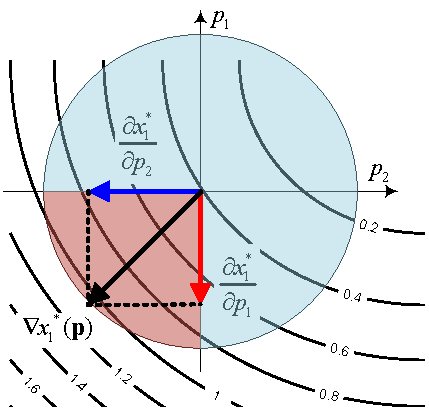
\includegraphics[width=0.4\textwidth]{5a_parameter_demo_ge0}
	\caption{Isocontours of the response surface ${x_1}^*(\mathbf{p})$ and transition rule $\mathbf{N}~\mathbf{J}^{\text T}(\mathbf{p})\mathbf{M} \ge \mathbf{0}$ in a two-dimensional parameters space}
	\label{fig:contourdemo}
\end{figure}

To illustrate Equation~(\ref{eq:transitionrulematrix}), a two-dimensional parameters space example is shown in Figure~\ref{fig:contourdemo}. 

The change agent vector $\mathbf{n}$ describes a quadrant (or hyper-octant in higher dimensions) in the parameters space that should contain the gradient vector $\nabla\hat{\mathbf{x}^*}(\mathbf{p})$. The sign of the gradient vector is modified by the monotonicity vector $\mathbf{m}$. Figure~\ref{fig:contourdemo} shows an example when $m_l\nabla\hat{{x_1}^*}(\mathbf{p}) \ge 0$ and lies within the quadrant defined by $\mathbf{n}$. Designs within the change agent quadrant and having gradients leading to an increase in their value are considered scalable.

In order to map scalable designs from the parameters space to the design space, the design space is resampled randomly and the transition rule (Equation~(\ref{eq:transitionrulematrix})) is checked for every sample $\mathbf{p}_o$. If $\mathbf{N}~\mathbf{J}^{\text T}(\mathbf{p}_o)\mathbf{M} \ge \mathbf{0}$ is satisfied then the corresponding design $\hat{\mathbf{x}^*}(\mathbf{p}_o)$ is retrieved and appended to a set of scalable solutions $\mathbf{X}_s$.

The procedure for obtaining the set of scalable optimal solutions is presented in Algorithm~\ref{algo:SODalgo}.

\begin{algorithm}
	\DontPrintSemicolon % Some LaTeX compilers require you to use \dontprintsemicolon instead
	\KwIn{
		Parameter space bounds $\mathbf{L}_p$ and $\mathbf{U}_p$, \ac{KS} response surface of parameters space $\hat{\mathbf{x}^*}(\mathbf{p})$, Jacobian of parameters space $\nabla\hat{\mathbf{x}^*}(\mathbf{p})$, Monotonicity matrix $\mathbf{M}$, Change agent matrix $\mathbf{N}$, \ac{LH} samples of parameters space $\left[\mathbf{p}_{1},\mathbf{p}_{2}, \cdots, \mathbf{p}_{o}\right]^{\text T}$
	}
	\KwOut{$\mathbf{X}_s$}		
	\For{$k \gets 1$ to $o$} {
		%				Populate possible points using LH and store them in $S_k$\;
		%				Update the RAM using built SM\;

		\If{$\mathbf{N}~\mathbf{J}^{\text T}(\mathbf{p}_k)\mathbf{M} \ge \mathbf{0}$} {
			Find design variables corresponding to parameters sample using response surface $\mathbf{x}^*(\mathbf{p}_k) = \hat{\mathbf{x}^*}(\mathbf{p_k})$\;
			Augment $\mathbf{X}_s \gets \mathbf{X}_s \cup \{ \mathbf{x}^*(\mathbf{p}_k) \} $\;
		}
		\Else{
			$\mathbf{X}_s \gets \mathbf{X}_s$\;
		}
	}
	\caption{Pseudo-algorithm for obtaining the set of scalable optimal designs $\mathbf{X}_s$}
	\label{algo:SODalgo}
\end{algorithm}

% --------------------------------- Numerical example ------------------------------------ %
\subsection{Numerical example for determining the scalable design set} \label{subsec:numex}

\begin{figure*}[h!]
	\centering
	\subfloat[Sampling effect \label{fig:nsamples_test}]{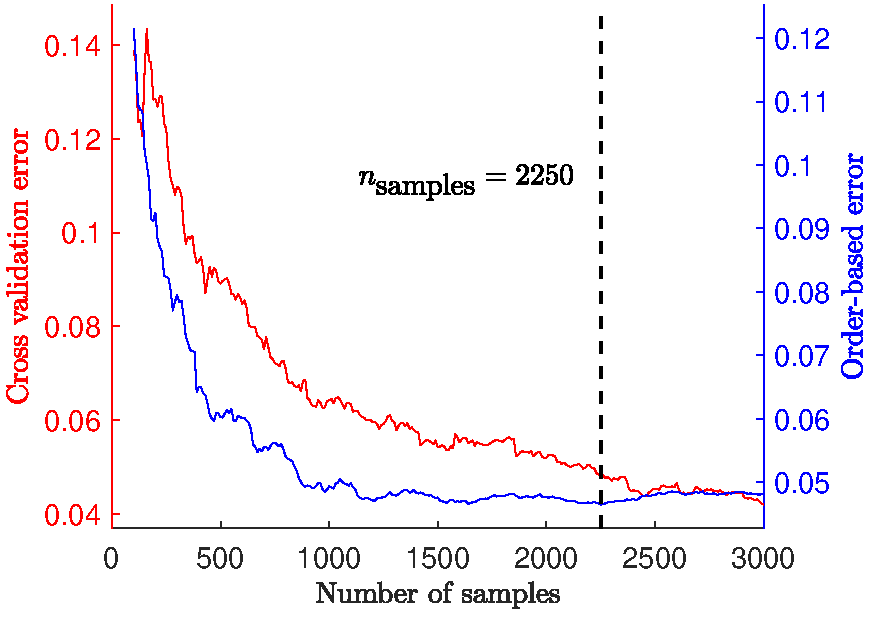
\includegraphics[width=0.4\textwidth]{OE_nsamples}} \hspace{0.07\textwidth}%
	\subfloat[Bandwidth effect \label{fig:bandwidth_test}]{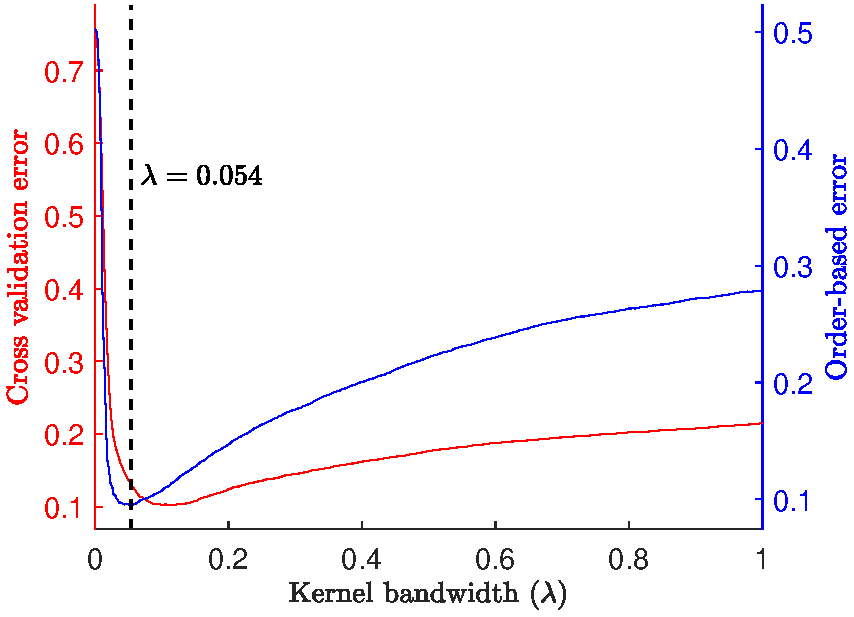
\includegraphics[width=0.4\textwidth]{OE_bandwidth}}
	\caption{Effect of number of training points and kernel bandwidth on order-based error}
	\label{fig:HPeffect}
\end{figure*}

\begin{figure*}[h!]
	\centering
	\subfloat[Test function \label{fig:testfunanalytical}]{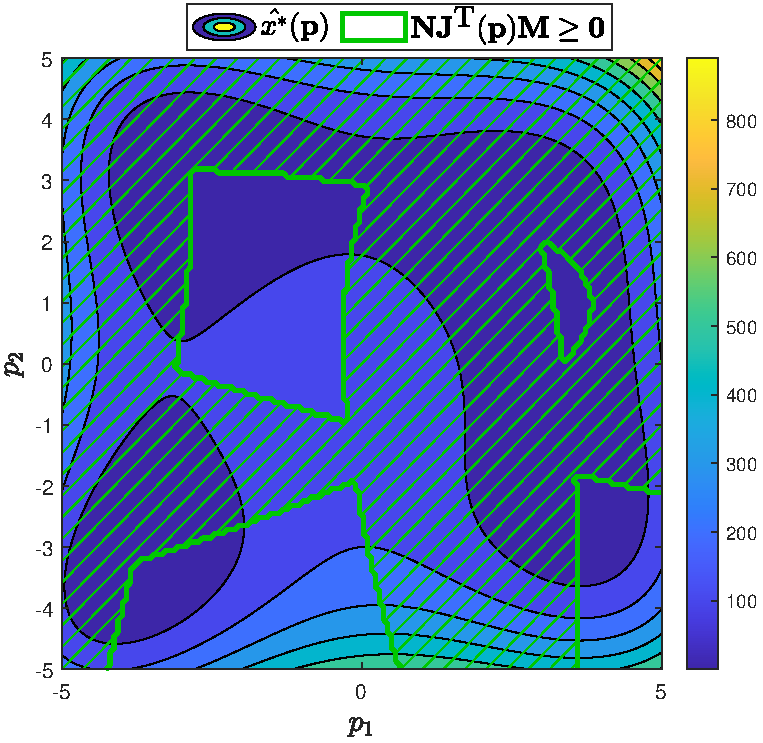
\includegraphics[width=0.4\textwidth]{test_problem}} \hspace{0.07\textwidth}%
	\subfloat[\ac{KS} approximation \label{fig:testfunKS}]{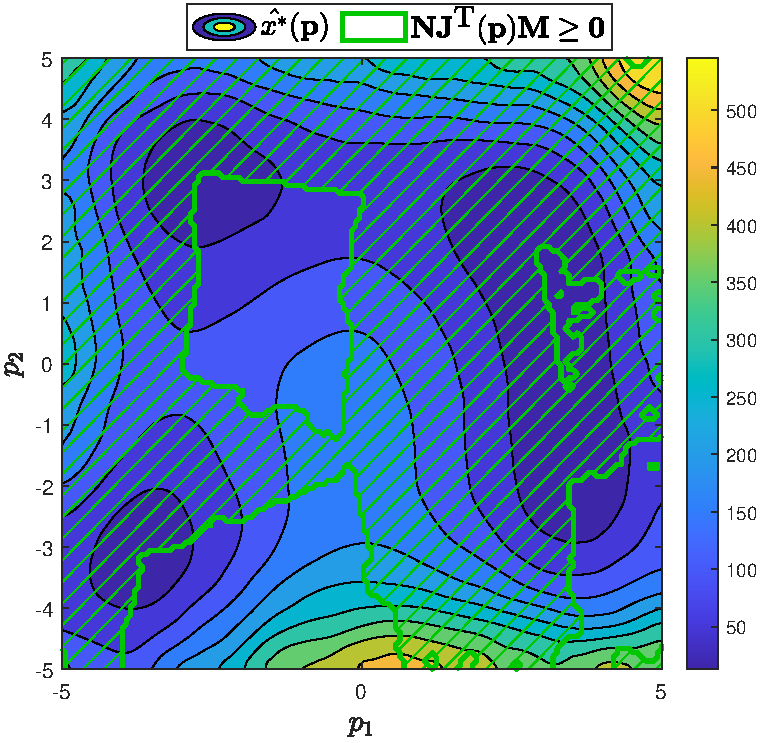
\includegraphics[width=0.4\textwidth]{test_problem_KS}}	
	\caption{Approximation of scalable set using \ac{KS} with non-scalable regions of the parameters space hatched}
	\label{fig:testfun}
\end{figure*}

We demonstrate the concepts related to constructing a \ac{KS} response surface to estimate the Jacobian using a numerical example. We also show how the estimated Jacobian can be used for identifying the scalable design set. Himmelblau's test function is used as it features multiple local minima. The test function and its Jacobian are
\begin{displaymath}
%	\begin{aligned}
		{x}^*(p_1,p_2) = ({p_1}^{2}+{p_2}-11)^{2}+({p_1}+{p_2}^{2}-7)^{2} 
		\end{displaymath}
		and
	\begin{displaymath}	
		\mathbf{J}(p_1,p_2) = \begin{bmatrix}
			4{p_1}({p_1}^2 + {p_2} - 11) + 2({p_1} + {p_2}^2 -7) \\ 
			2({p_1}^2 + {p_2} - 11) + 4{p_2}({p_1} + {p_2}^2 -7) 
	\end{bmatrix},
	\end{displaymath}
	respectively.% (i.e., $\mathbf{p} = \left[p_1,p_2\right]$).

We approximate the response surface for this function via \ac{KS} to obtain $\hat{{x}^*}(\mathbf{p)}$. For this example we set the change agent vector as $\mathbf{n} = \left[1~-1\right]$ and the monotonicity vector as $\mathbf{m} = \left[1\right]$. The test function is sampled via \acp{LH} to create the training data for the \ac{KS} model. We evaluate the transition rule $\mathbf{N}~\mathbf{J}^{\text T}(\mathbf{p})\mathbf{M} \ge \mathbf{0}$ defining the scalable set using the analytical and estimated Jacobian. The estimated Jacobian was obtained by differentiation of the \ac{KS} basis functions. A portion of the \ac{LH} samples are reserved for use as a validation set and are not used to train the \ac{KS} model. The cross-validation error reflects the classification accuracy of the \ac{KS} response surface at the validation points as part of the true scalable set obtained from the analytical Jacobian.

In addition, we use the order-based error proposed in \cite{Audet2018} since it does not rely on comparisons with the true scalable set (which is not available in real problems). It is computed by checking how accurately the response surface model orders the validation points. It is calculated as 
%
\begin{equation}
    \label{eq:oeobjective}
	\varepsilon_{OE} = \frac{1}{n_{cv}^2} \sum_{i=1}^{n_{cv}} \sum_{l=1}^{n_{cv}} \theta\left(\mathbf{x}^*(\mathbf{p}_i) - \mathbf{x}^*(\mathbf{p}_l),\hat{\mathbf{x}^*}(\mathbf{p}_i) - \hat{\mathbf{x}^*}(\mathbf{p}_l)\right),
\end{equation}
%
where $n_{cv}$ is the number of validation points. The function $\theta$ is defined as
%
\begin{equation}
    \label{eq:theta}
    \theta\left(a,b\right) = \left(a \le 0\right)~\textrm{xor}~\left(b \le 0\right),
\end{equation}
%
where xor is the logical \textit{exclusive or} operator.
Figure~\ref{fig:HPeffect} shows the effect of the number of training points ($n_{\textrm{samples}}$) and the bandwidth ($\lambda$) on the cross validation and order-based errors.

It can be seen that there is a unique combination of $n_{\textrm{samples}}$ and $\lambda$ that yield the best response surface for assessing scalability in the parameters space. The true and estimated scalable sets are shown in Figure~\ref{fig:testfun}. The \ac{KS} model used for the estimation is trained using 2305 training samples and a bandwidth of $\lambda = 0.054$.
Figure~\ref{fig:testfun} shows that \ac{KS} is capable of capturing the scalable set despite underestimating the magnitude of the test function. Figure~\ref{fig:HPeffect} shows that the order-based error is a good indication of the prediction accuracy of the \ac{KS} model for the scalable set. As a result, the \ac{KS} parameters and number of training points can be determined by minimizing the order-based error.

In summary, the proposed methodology consists of two design filters that determine a set of scalable optimal designs to be considered for further development. The first filter retains designs that dominate in terms of performance throughout the parameters space (set of parametric optimal designs $\mathbf{X}^*$). The second filter retains designs that are scalable by remanufacturing (scalable design set $\mathbf{X}_s$). The number of samples for the \ac{KS} response surface is chosen such that the order-based error is minimized with respect to a validation set. The methods developed in this section are now applied to an industrial case study.

The proposed methodology, is presented as a flow diagram in Figure~\ref{fig:SBDmethods}

\begin{figure}[h]
	\centering
	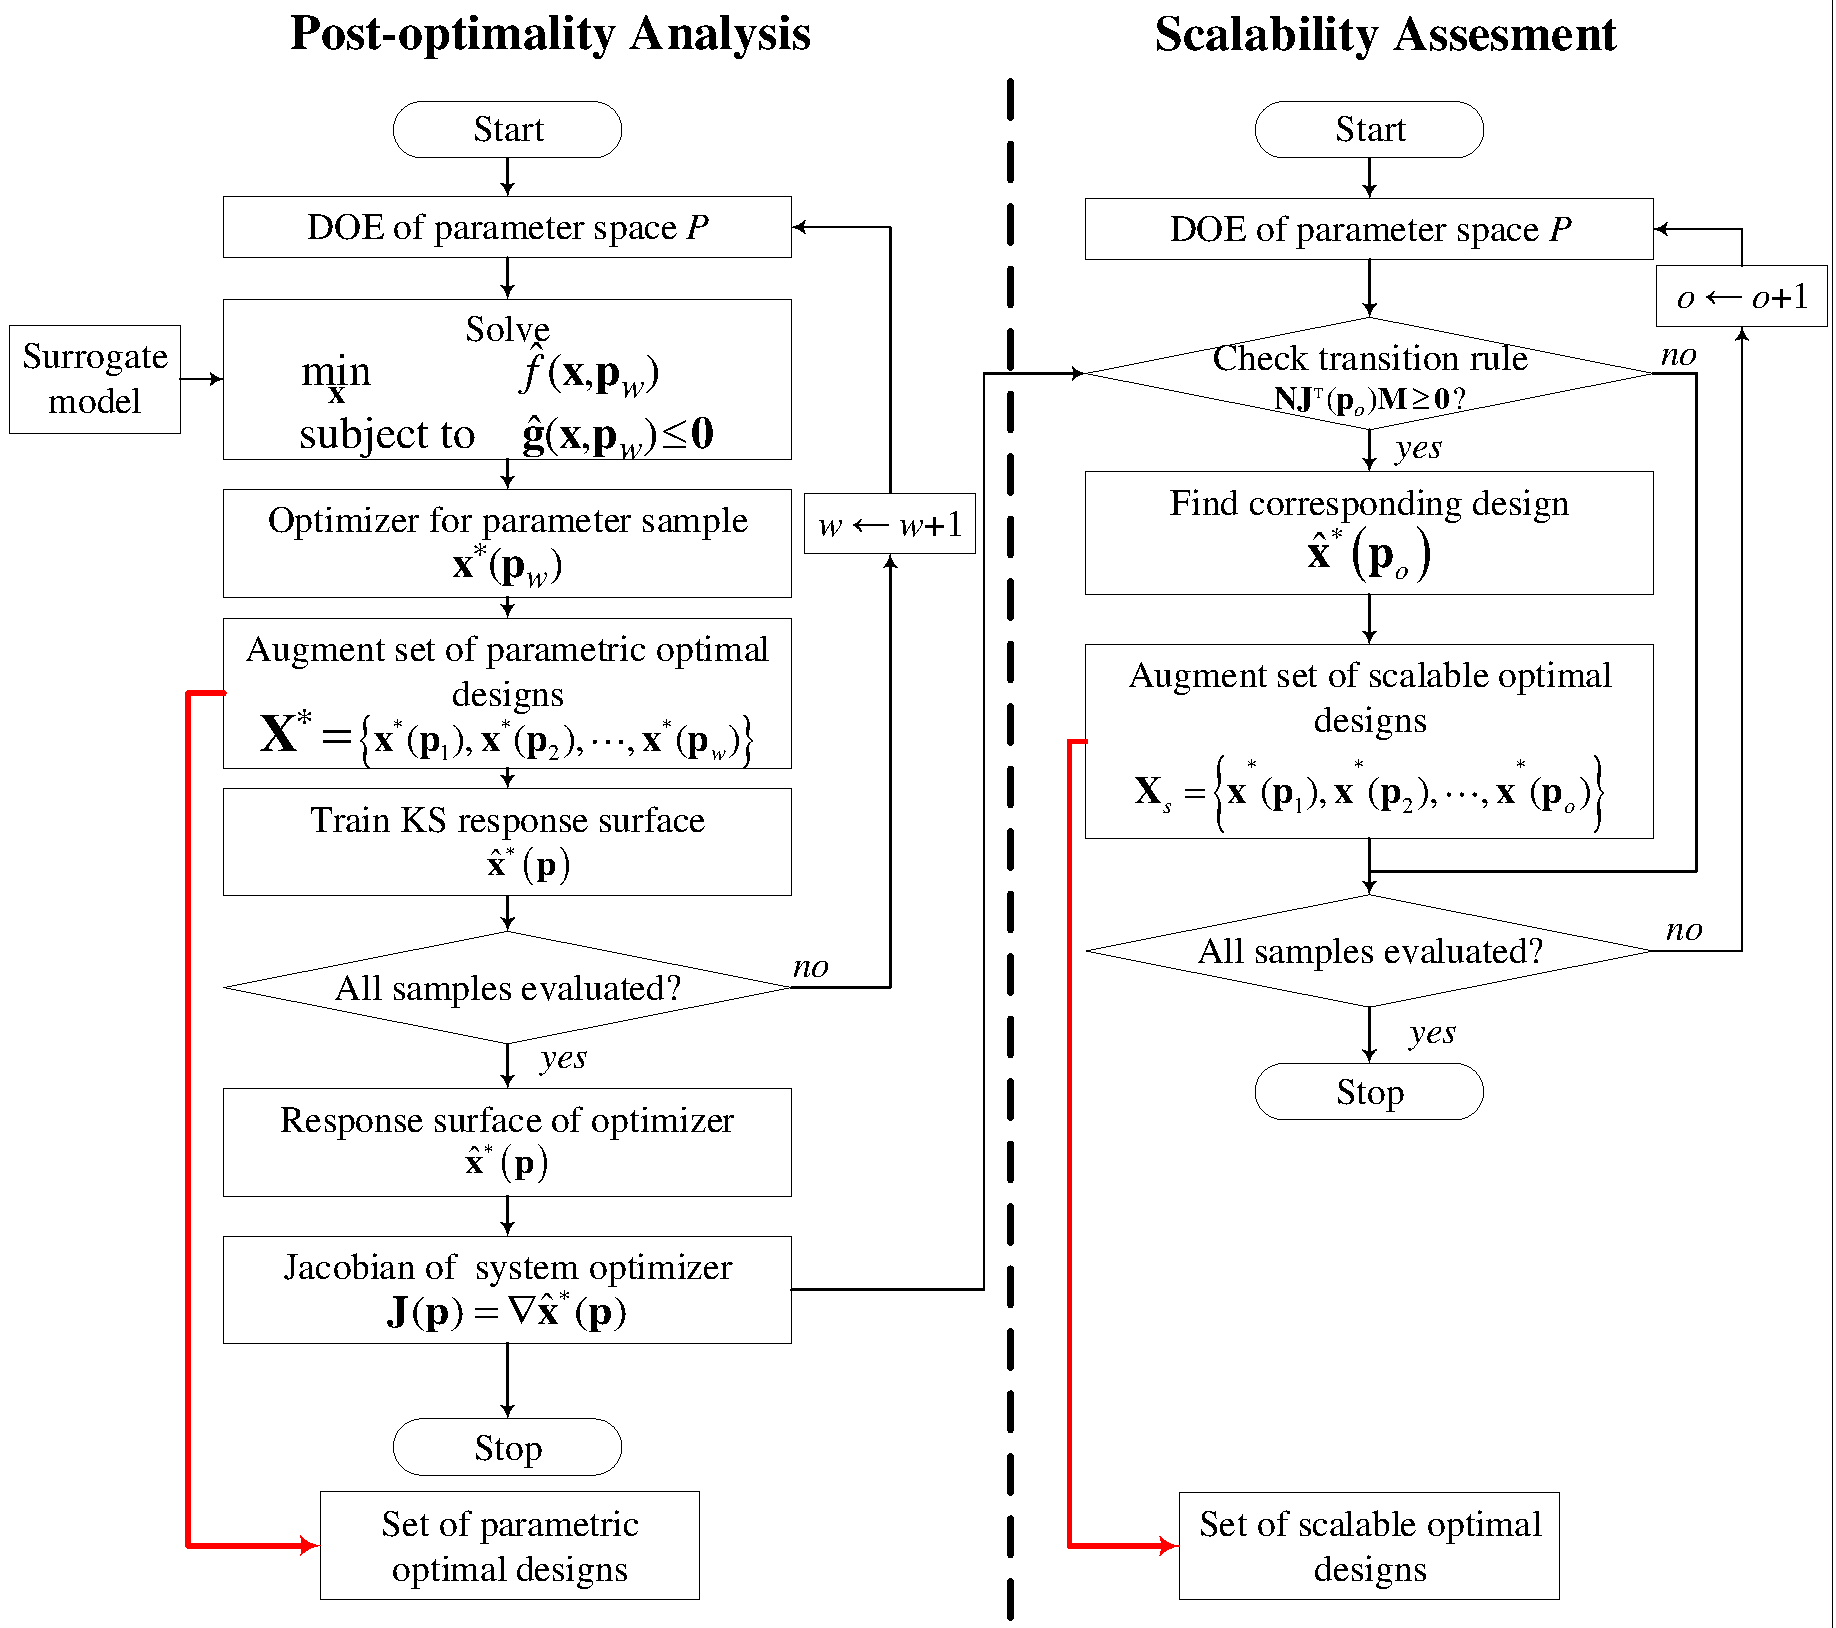
\includegraphics[width=.95\textwidth]{5_methodology_V2.pdf}
	\caption{ \label{fig:SBDmethods} Set-based design space reduction methodology}
\end{figure}

%============================ CASE STUDY =======================================%
\section{Application example: aeroengine component remanufacturing} \label{sec:SBDusecase}

The \ac{TRS} structural aeroengine component described in Chapter~\ref{ch:thermomechanical} is used to demonstrate the methodology for obtaining scalable optimal designs when considering it for remanufacturing.

The safety factor against low-cycle fatigue is computed using the model in Section~\ref{subsec:fatigueanalysis} as a structural performance requirement.

% Model summary
The design variables for this problem shown in Figure~\ref{fig:TRSoverview} are extracted from Table~\ref{table:modelinputs} and listed in Table~\ref{table:SBDvariables} along with their monotonicity.

\begin{table}[h!]
\centering
\renewcommand{\arraystretch}{1.0}% Wider
\footnotesize\addtolength{\tabcolsep}{-5pt}
\caption{Design variables ${\textbf{x}}$}
\label{table:SBDvariables}
	\begin{tabular}{lcc>{\centering\arraybackslash}p{1cm}>{\centering\arraybackslash}p{1cm}>{\centering\arraybackslash}p{1cm}}
		\hline\hline
		\bf Design variable & \bf Notation & \bf Units & \bf Lower bound & \bf Upper bound & \bf Mono- tonicity\\
		\hline
		Stiffener axial position & $x_1$ & mm & 37 & 145 & 0 \\
		Stiffener thickness  & $x_2$ & mm & 2 & 10 & 1 \\
		Stiffener width & $x_3$ & mm & 10 & 40 & 1  \\
		Laser Power & $P_{\textrm{laser}}$ & W & 3,500 & 4,000 & 0\\ 
		%Laser beam radius & ${r_l}$ & mm & 12.6 & 16.0 \\ 
		%Scanning speed& ${V}$ & mm/s & 4.0 & 4.6 \\ 
		\hline\hline
	\end{tabular}
\end{table}

Similarly, the design parameters relevant to the problem in this chapter are extracted from Table~\ref{table:modelinputs} and are listed in Table~\ref{table:SBDparametervar} along with their change agent values.

\begin{table}[h!]
\centering
\renewcommand{\arraystretch}{1.0}% Wider
\footnotesize\addtolength{\tabcolsep}{-5pt}
\caption{Design parameters $\textbf{p}$}
\label{table:SBDparametervar}
\begin{tabular}{lcc>{\centering\arraybackslash}p{2cm}>{\centering\arraybackslash}p{1cm}}
\hline\hline
\bf Parameter    & \bf Notation & \bf Units & \bf Range  &\bf Change agent\\ \hline
Internal pressure load  & ${P}_{\textrm{load}}$ & MPa & $2 \pm 0.5$ & 1\\ 
Deposit melting point & $T_m$ & $^o$C & $1,500 \pm 100$ & -1\\
Substrate base width & $W_{\textrm{total}}$ & mm & $137.5 \pm 17.5$ & -1\\
\hline\hline
\end{tabular}
\end{table}

The remanufacturing model variables and parameters given by Tables~\ref{table:SBDvariables} and \ref{table:SBDparametervar} respectively are used for the formulation of the optimization problem for \ac{SBD} in the following section. 

% --------------------------- parametric optimal design space reduction ------------------------------ %
\subsection{Problem formulation} \label{subsec:SBDproblemformulation}

The design optimization problem is formulated as 
\begin{equation}
	\label{eq:SBCEopt}
	\begin{aligned}
		& \min_{\mathbf{x} = \left[x_1,x_2,x_3,P_{\textrm{laser}}\right]^{\text T}}
		& & f(\mathbf{x};\mathbf{p}) = -n_{\textrm{safety}}(P_{\textrm{load}})\\
		& \text{subject to}
		& & g_1(\mathbf{x};\mathbf{p}) = x_3 + x_1 - W_{\textrm{total}} \le 0\\
		& & & g_2(\mathbf{x};\mathbf{p}) = T_m - T_\textrm{deposit} \le 0,
		% & & & g_3(\mathbf{x}) = U_{\textrm{res}}(\mathbf{x}) - U_{\textrm{max}} \le 0\\
%		& \text{where}
%		& & \mathbf{x}^{\text T} = \left[x_1,x_2,x_3,P\right]
	\end{aligned}
\end{equation}
where $n_{\textrm{safety}}$ is the safety factor against low cycle fatigue or first cycle yielding for the load case. The constraints pertain to the substrate width on the outer casing (the region where deposition is permitted) and the melting temperature of the deposit material needed to consolidate the material.

% --------------------------- Design space reduction to parametric optimal design set ------------------------------ %
\subsection{Parametric optimal design results} \label{subsec:reduceddesignspace}

The design optimization problem in Equation~(\ref{eq:SBCEopt}) is solved using the \ac{MADS} algorithm. We use the \texttt{OrthoMADS} implementation provided by the \texttt{NOMAD} algorithm \cite{LeDigabel2011}. The termination criterion for \ac{MADS} was the minimum mesh size (defined by Audet and Dennis \cite{Audet2006a}) reached in the virtually discretized design variable space. Non-opportunistic latin hypercube search was used during the search step. A progressive barrier approach was used for handling constraints \cite{Audet2009}. This choice of algorithm is motivated by the possible non-existence of gradients or the inability to approximate them with reasonable computational cost and warranted due to its rigorous convergence properties.

As described earlier, \acp{LH} are used to sample the design and parameters spaces defined by the bounds and ranges of the design variables and parameters, respectively (see Tables 
~\ref{table:SBDvariables} and \ref{table:SBDparametervar}).

For our numerical investigations, the design optimization problem is solved for 1200 \ac{LH} samples of the parameters space to obtain a set of parametric optimal design solutions. Up to 900 samples are used as a training set for the \ac{KS} model, while the remaining 300 are reserved for use as a validation set to check the order-based error.

The effect of the parameters on the optimizer is illustrated by 3 sample results shown in Figure~\ref{fig:SBD1sens2P1} (see Table~\ref{table:optresults}).

\begin{figure*}%[t]
	\centering
	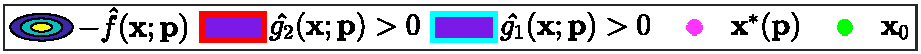
\includegraphics[width=0.65\textwidth]{9_f1_legend} \vspace{-0.02\textwidth}\\
	\subfloat[$\mathbf{p}_1$ \label{fig:p1}\label{fig:9a}]{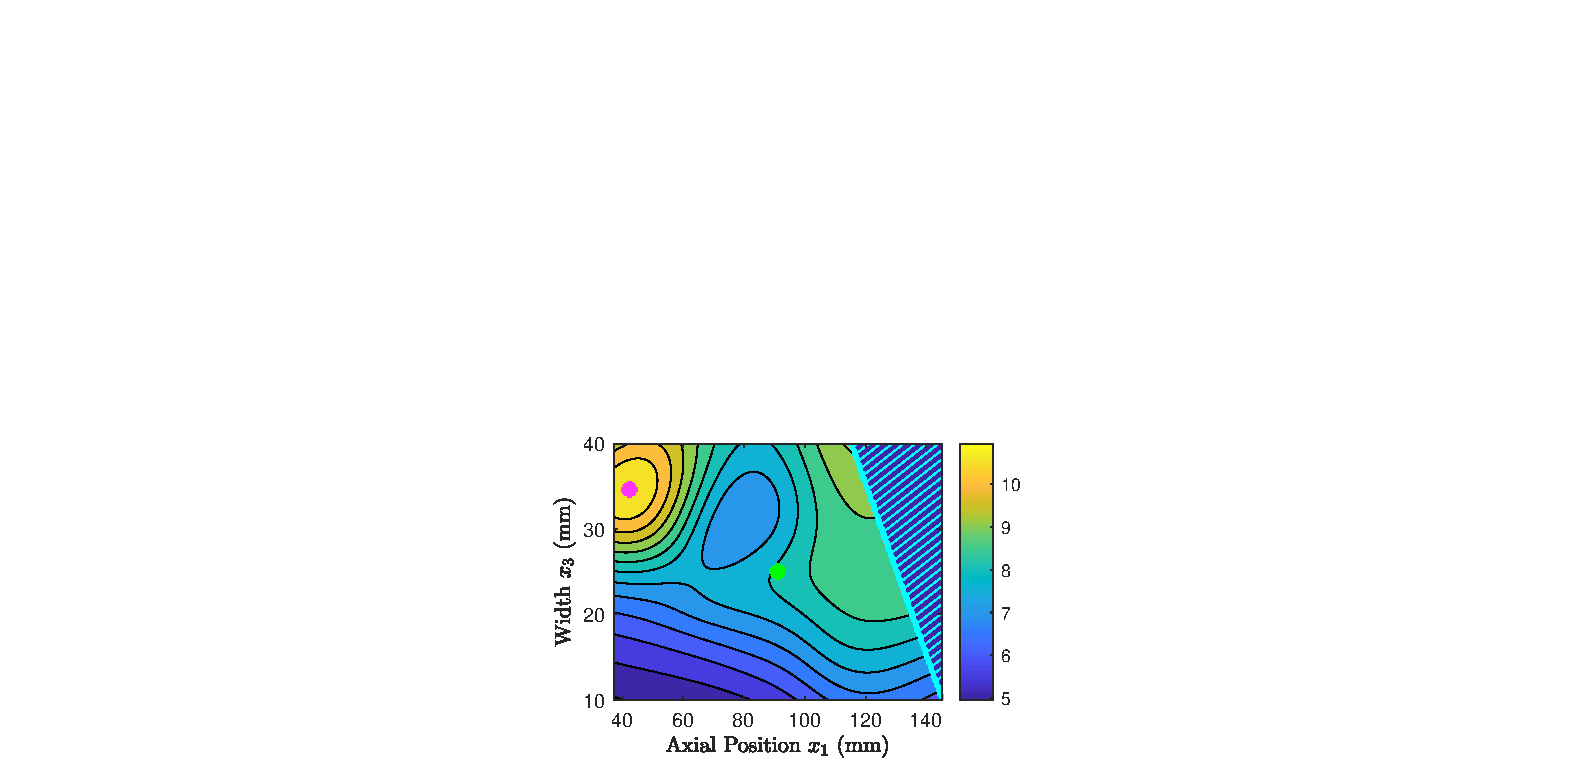
\includegraphics[height=0.21\textwidth]{9a_f1_1_p1}} \hspace{0.03\textwidth}%
	\subfloat[$\mathbf{p}_2$ \label{fig:p2}\label{fig:9b}]{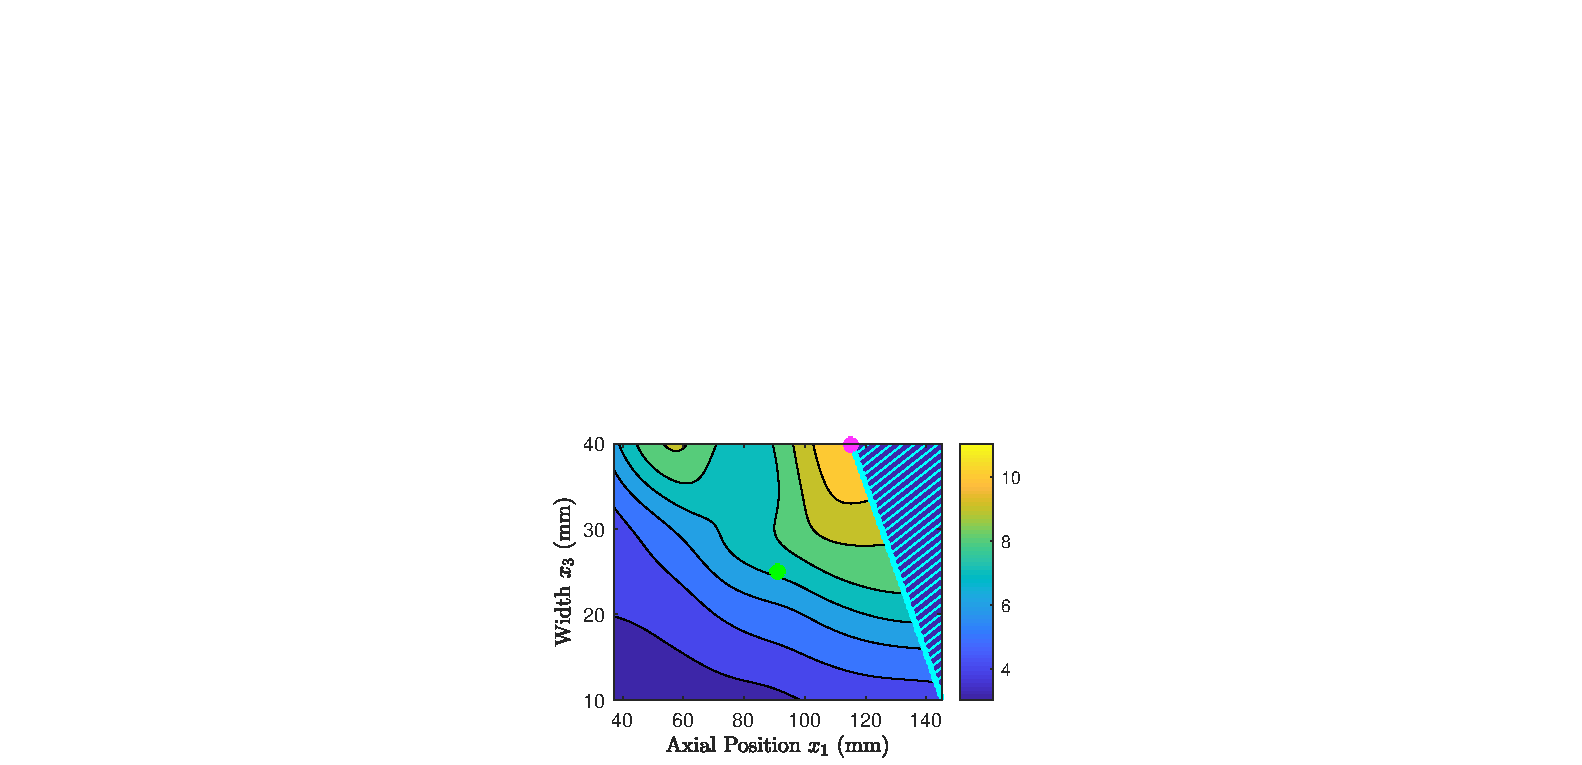
\includegraphics[height=0.21\textwidth]{9b_f1_1_p2}} \hspace{0.03\textwidth}%
	\subfloat[$\mathbf{p}_3$ \label{fig:p3}\label{fig:9c}]{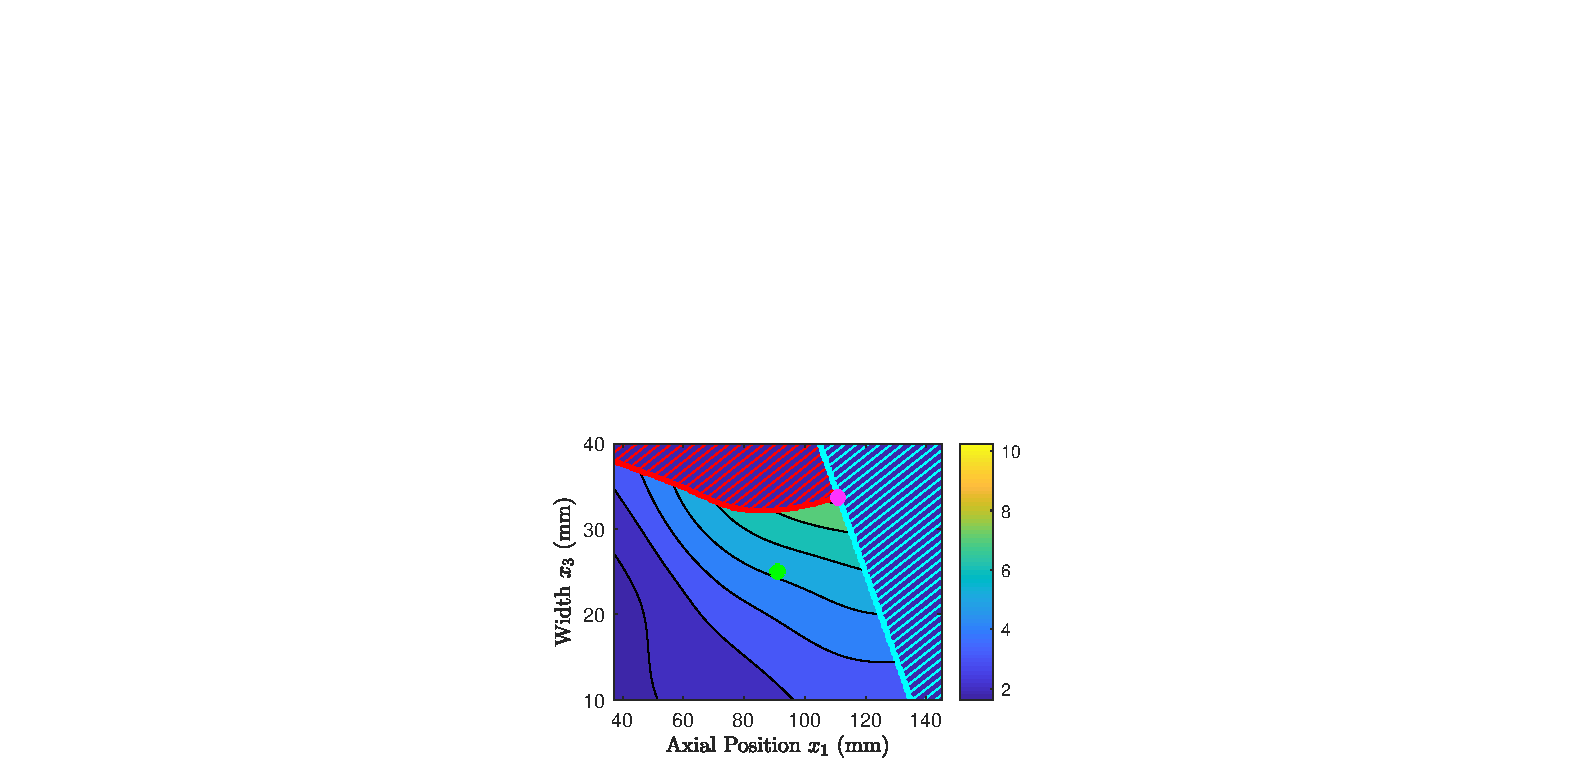
\includegraphics[height=0.21\textwidth]{9c_f1_1_opt}}
	\caption{Three sample parametric optimal designs; $x_0$ denotes the baseline design}
	\label{fig:SBD1sens2P1}
\end{figure*}
\begin{table*}[h!]
\centering
\renewcommand{\arraystretch}{1.0}% Wider
\small\addtolength{\tabcolsep}{-5pt}
\caption{Sample optimization problem results}
\label{table:optresults}
\begin{tabular}{cC{1.2cm}C{1.2cm}C{1.2cm}C{1.2cm}|C{1.2cm}C{1.2cm}C{1.2cm}|C{1.2cm}C{1.2cm}C{1.2cm}}
\toprule\toprule
\multirow{5}{1cm}{\textbf{Result}} & \multirow{5}{1cm}{\centering\textbf{Units}} & \multicolumn{9}{c}{\textbf{Parameters}}\\ \cline{3-11}
 & & \multicolumn{3}{c}{$\mathbf{p}_1$} & \multicolumn{3}{c}{$\mathbf{p}_2$} & \multicolumn{3}{c}{$\mathbf{p}_3$} \\ \cline{3-11}
 & & ${P}_{\textrm{load}}$ & $T_m$ & $W_{\textrm{total}}$ &  ${P}_{\textrm{load}}$ & $T_m$ & $W_{\textrm{total}}$ &  ${P}_{\textrm{load}}$ & $T_m$ & $W_{\textrm{total}}$ \\
 & & (MPa) & ($^o$C) & (mm) & (MPa) & ($^o$C) & (mm) & (MPa) & ($^o$C) & (mm) \\
 & & 1.87 & 1,400 & 155 &2.08 & 1,400 & 155 &  2.3973 & 1,427 & 145 \\
\hline
$x_1^*$ & mm & \multicolumn{3}{c|}{42.2} & \multicolumn{3}{c|}{115.1} & \multicolumn{3}{c}{110.9}\\
$x_2^*$ & mm & \multicolumn{3}{c|}{10.0} & \multicolumn{3}{c|}{9.0} & \multicolumn{3}{c}{8.8}\\
$x_3^*$ & mm & \multicolumn{3}{c|}{34.7} & \multicolumn{3}{c|}{39.9} & \multicolumn{3}{c}{33.7}\\
${P_{\textrm{laser}}}^*$ & W & \multicolumn{3}{c|}{3,500} & \multicolumn{3}{c|}{3,770} & \multicolumn{3}{c}{3,991}\\
$g_1(\mathbf{x}^*)$ & mm & \multicolumn{3}{c|}{-78.1} & \multicolumn{3}{c|}{0 (active)} & \multicolumn{3}{c}{0 (active)}\\
$g_2(\mathbf{x}^*)$ & $^o$C & \multicolumn{3}{c|}{-393} & \multicolumn{3}{c|}{-381} & \multicolumn{3}{c}{0 (active)}\\
$f(\mathbf{x}^*)$ & - & \multicolumn{3}{c|}{-11} & \multicolumn{3}{c|}{-11} & \multicolumn{3}{c}{-8}\\
\toprule\toprule
\end{tabular}
\end{table*}
These 3 samples have been chosen to include one interior optimal design (Figure~\ref{fig:9a}), one boundary optimal design with one active constraint ((Figure~\ref{fig:9b}), and one boundary optimal design with two active constraints (Figure~\ref{fig:9c}).
The optimizers obtained by sampling the parameters space are used to construct a convex hull to quantify the size of the set of parametric optimal designs. The \texttt{qhull} algorithm was used to construct the 4-dimensional polygon (polytope) characterizing the convex hull \cite{Barber2002}.

% --------------------------- Scalable Design Space ------------------------------ %
\subsection{Scalable optimal design results} \label{subsec:scalabledesignspace}

Of the 900 parametric optimal designs obtained by solving the optimization problem for different parameter values, 592 samples were used to construct a response surface that can predict a parametric optimal design for other parameter values. As explained in Section~\ref{subsec:numex} the order-based error relative to a validation set was minimized to determine the number of training samples. The kernel bandwidth ($\lambda$) was determined to be 0.71. This result is shown in Figure~\ref{fig:HPeffectSBD}.

Designs meeting scalability requirements in the parameters space are identified using the scalability constraint in Section~\ref{subsec:SBDfAM}. The monotonicity vector is defined as $\mathbf{m} = [0~1~1~0]^{\text T}$ for the variables in Table~\ref{table:SBDvariables}. The {change agent} vector is defined as $\mathbf{n} = [1~-1~-1]^{\text T}$. As an illustrative example, the two-dimensional projections of the parameters space for the optimal width design variable are depicted in Figure~\ref{fig:parameterspacescaled}.
\begin{figure*}%[t]
	\centering
	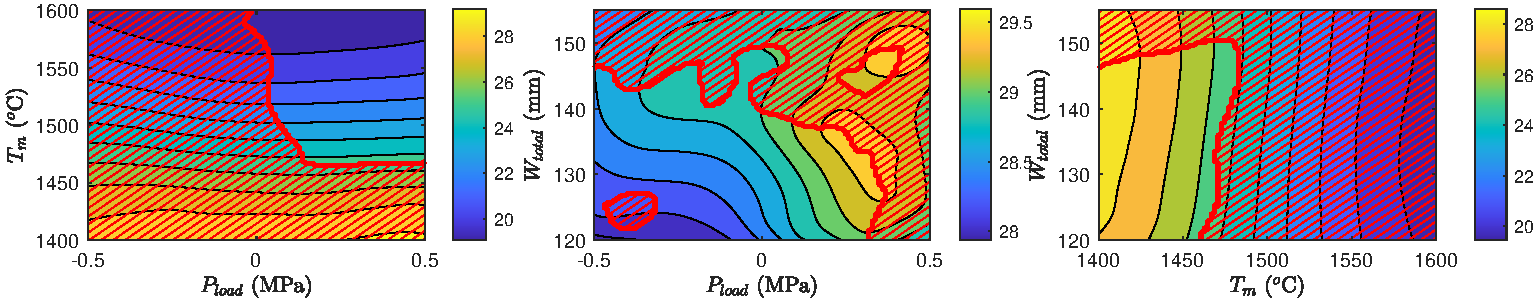
\includegraphics[width=1\textwidth]{12_parameter_space_scaled_V2.pdf} %12_parameter_space_scaled.pdf
	\caption{ \label{fig:parameterspacescaled} Projections of the optimal width design variable $\hat{x_3}^{*}$ with non-scalable regions of the parameters space hatched}
\end{figure*}
\begin{figure*}[h!]
	\centering
	\subfloat[Sampling effect \label{fig:nsamples}]{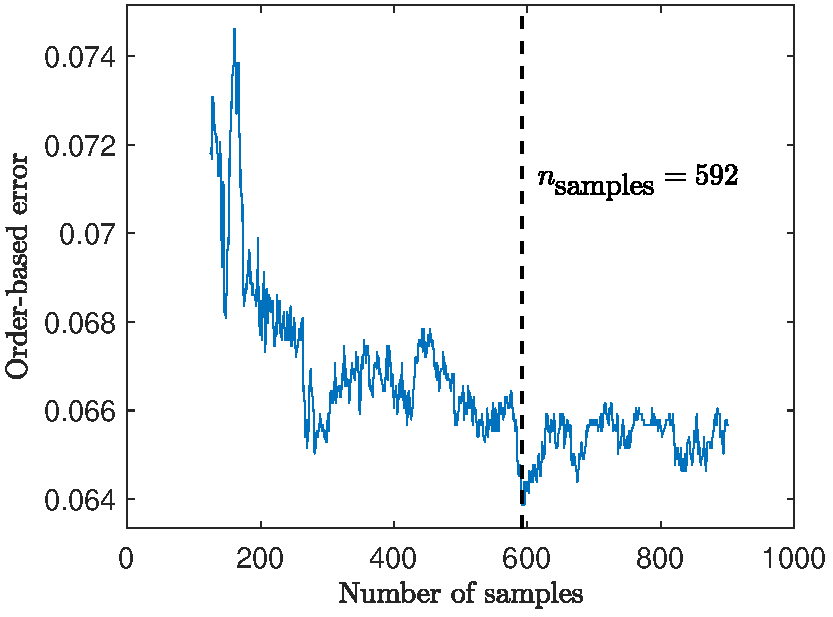
\includegraphics[width=0.4\textwidth]{OE_nsamples_SBD}} \hspace{0.02\textwidth}%
	\subfloat[Bandwidth effect \label{fig:bandwidth}]{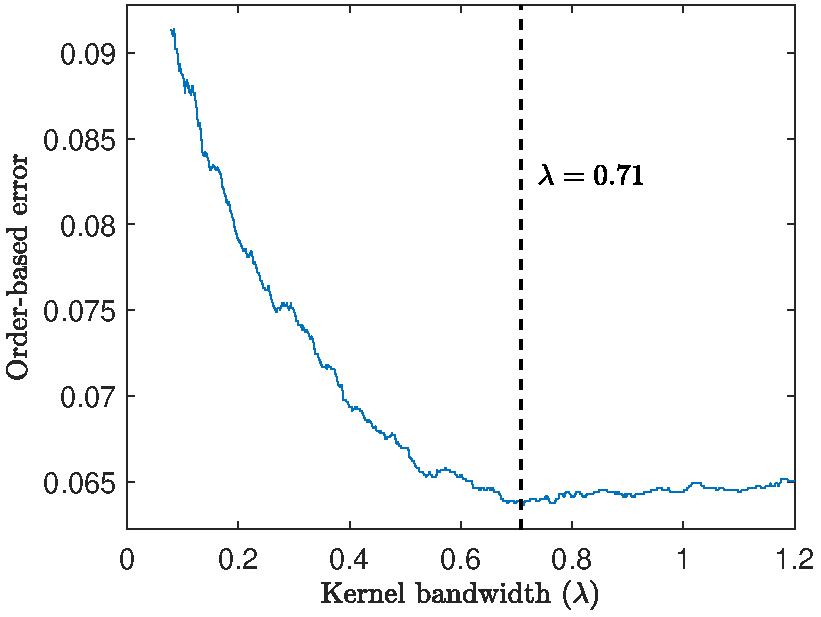
\includegraphics[width=0.4\textwidth]{OE_bandwidth_SBD}}	
	\caption{Effect of number of training points and kernel bandwidth on order-based error}
	\label{fig:HPeffectSBD}
\end{figure*}

The scalability transition rule results in pockets within the parameters space that can be mapped back to design space by evaluating the optimizer response surface within these pockets. The parameters space is sampled using a full factorial grid and designs meeting the scalability constraint are tabulated and projected on the design space in Figure~\ref{fig:FullM}.
\begin{figure*}[h!]
	\centering
	\subfloat[$\mathbf{m} = [0~1~1~0{]}^{\text T}$, $\mathbf{n} = [1~-1~-1{]}^{\text T}$ \label{fig:FullM}]{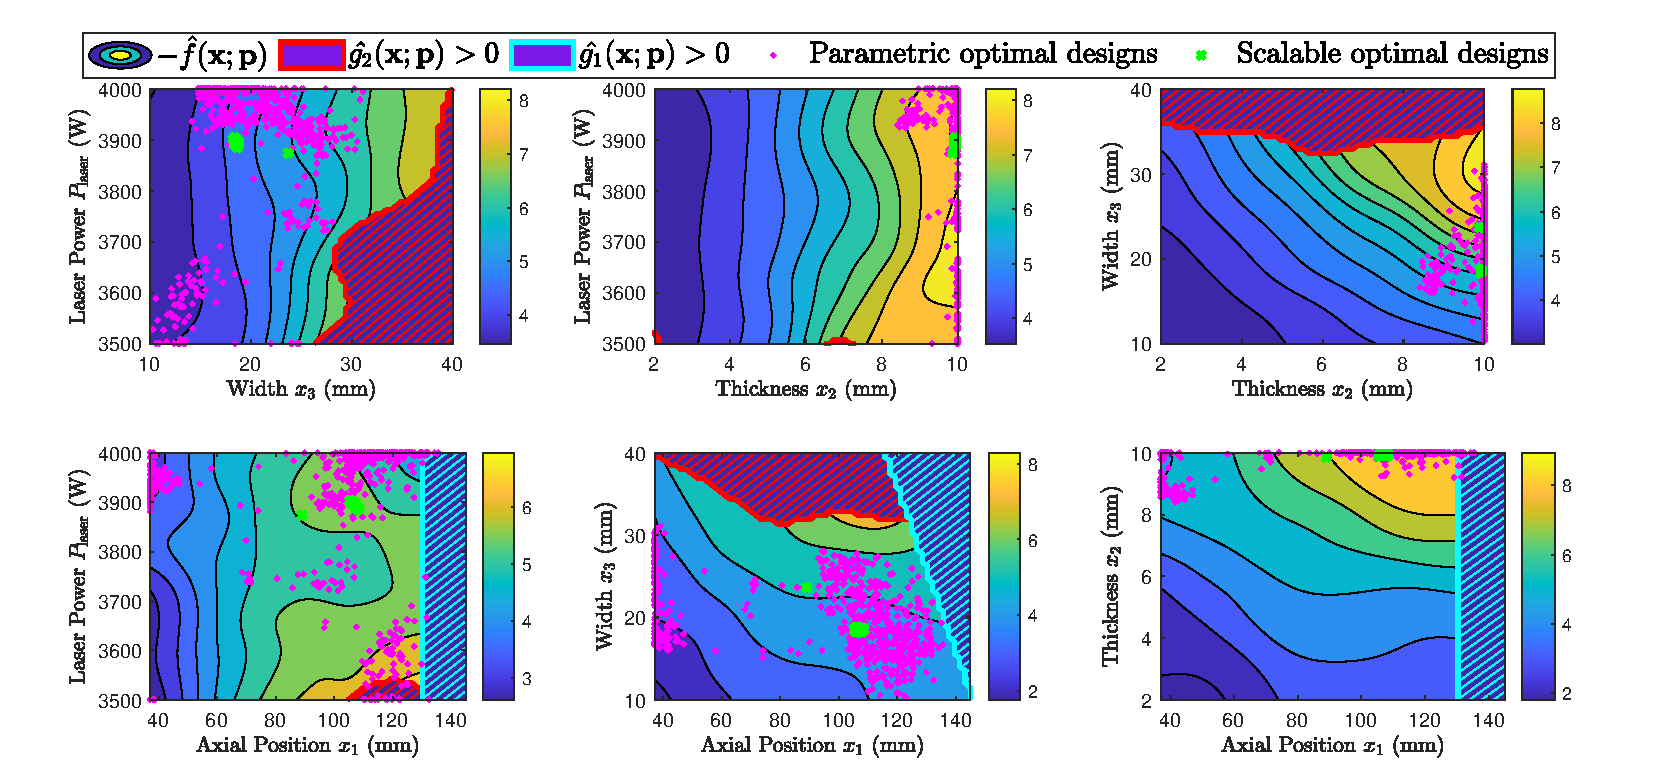
\includegraphics[width=1\textwidth]{8_design_space_V3.pdf}}\\
	\subfloat[$\mathbf{m} = [0~0~1~0{]}^{\text T}$, $\mathbf{n} = [1~-1~-1{]}^{\text T}$ \label{fig:RelaxedM}]{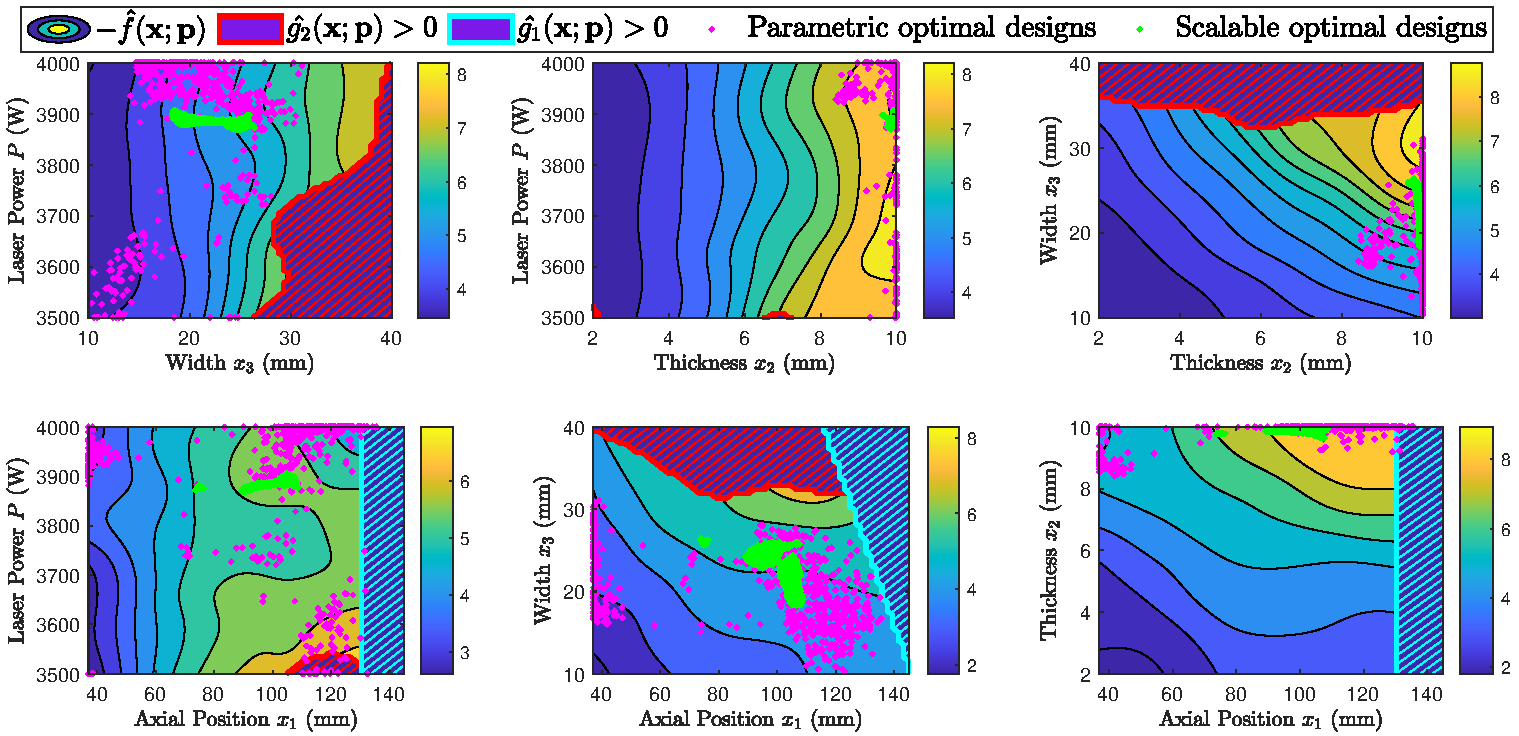
\includegraphics[width=1\textwidth]{8_design_space_V4.pdf}}	
	\caption{Safety factor in the feasible design space as a function of design variables for different monotonicity vectors}
	\label{fig:designspace}
\end{figure*}

The convex hull formed by the scalable optimal designs is considerably smaller in volume than that formed by the set of parametric optimal designs.

 The set of scalable optimal designs can be enlarged to include more designs by relaxing some of the scalability constraints. We relax all the constraints with respect to the thickness design variable $x_2$ by setting the monotonicity with respect to $x_2$ to $0$. The monotonicity vector becomes $\mathbf{m} = [0~0~1~0]^{\text T}$. The result of this relaxation is shown in Figure~\ref{fig:RelaxedM}.

Adhering to scalability constraints allows designers the flexibility to scale designs as parameters evolve even after commitment by considering remanufacturing scenarios. Figure~\ref{fig:parameterspacescaled} shows this scenario as the contours of $\hat{x_3}^{*}$ increase in value for any vector contained within the change agent hyperoctant as defined by $\mathbf{n}$.

% --------------------------- Design space variability ------------------------------ %
\subsection{Design set variability and comparison} \label{subsec:dspacevar}

Having generated the feasible design set, the set of parametric optimal designs, and the set of scalable optimal designs for the \ac{TRS} remanufacturing problem, some comparisons can be made.
Several metrics exist in the literature for comparing the variability of a design solution set generated by parametric optimal design tools such as those formulated in this thesis. The volume of the convex hull provides a good perception of design variability provided that there are sufficient points to construct the polytope characterizing the convex hull \cite{Brown2019}. The convex hull volume was used to compare the reduction in the design sets as our methodology was applied to the \ac{TRS} problem. The lower and upper bounds (LB and UB, respectively) of the ranged set containing each solution set are also found. They are used to compute the volume of the bounding hyper-rectangle. The hyper-rectangle volume provides a benchmark against the ranged set representation used for previous \ac{SBD} studies \cite{Qureshi2014, Nahm2005, Olewnik2004,Liu2008,Suh2007}.

% Case with one active variable
\begin{table*}[h!]
	\centering
	\small\addtolength{\tabcolsep}{-5pt}
	\caption{Design space comparison results}
	\label{table:designvariability}
	\begin{tabular}{l|C{1.2cm}C{1.2cm}|C{1.2cm}C{1.2cm}|C{1.2cm}C{1.2cm}|C{1.2cm}C{1.2cm}}
		\toprule\toprule
		\multirow{2}{1cm}{\textbf{Quantity}} & \multicolumn{2}{c|}{Feasible design} & \multicolumn{2}{c|}{Set of parametric} & \multicolumn{4}{c}{Scalable design set}\\
		& \multicolumn{2}{c|}{space} & \multicolumn{2}{c|}{optimal designs} & \multicolumn{2}{c|}{$\mathbf{m} = [0~1~1~0{]}^{\text T}$} & \multicolumn{2}{c}{$\mathbf{m} = [0~0~1~0{]}^{\text T}$}\\
		&  &  &  &  & \multicolumn{2}{c|}{$\mathbf{n} = [1~-1~-1{]}^{\text T}$} & \multicolumn{2}{c}{$\mathbf{n} = [1~-1~-1{]}^{\text T}$}\\
		& LB & UB & LB & UB & LB & UB & LB & UB\\
		\hline
		$x_1$ & 37 & 145 & 37 & 136 & 88.9 & 108.6 & 73.7 & 108.7\\
		$x_2$ & 2 & 10 &  8.4 & 10 & 9.8 & 9.9 & 9.6 & 9.9 \\
		$x_3$ & 10 & 40 & 10.3 & 31.1 & 18.3 & 23.7 & 18.3 & 26.4 \\
		$P_{\textrm{laser}}$ & 3500 & 4000 & 3500 & 4000 & 3874 & 3904 & 3869 & 3907 \\
		\hline
		$V_{\textrm{hyper-rectangle}}$ & \multicolumn{2}{c}{1} & \multicolumn{2}{c}{0.13} & \multicolumn{2}{c}{0.0016} & \multicolumn{2}{c}{0.0025}\\
		$V_{\textrm{convhull}}$ & \multicolumn{2}{c}{0.77} & \multicolumn{2}{c}{0.028} & \multicolumn{2}{c}{$6.3\times10^{-9}$} & \multicolumn{2}{c}{$1.04\times10^{-5}$}\\
		Relative volume & \multicolumn{2}{c}{77\%} & \multicolumn{2}{c}{2.8\%} & \multicolumn{2}{c}{$6.3\times10^{-7}\%$} & \multicolumn{2}{c}{0.00104\%}\\
		\toprule\toprule
	\end{tabular}
\end{table*}

Table~\ref{table:designvariability} summarizes the results of this comparison. It can be seen that a significant reduction of the design space was caused by each set-based filter step of our methodology. This is because smaller values for the laser power $P_{\textrm{laser}}$ and thickness $x_2$ resulted in consistently suboptimal designs with respect to performance. However, among the scalable designs many featured axial positions ($x_1$) and widths ($x_3$) near the upper and lower bounds for each variable respectively. This is due the positive monotonicity of the volume with respect to $x_3$. Such designs have the greatest potential for scalability. The relative volume of the convex hull to that of the design space is calculated in the last row of the table. The design space volume was normalized to 1 for ease of comparison. Feasible solutions comprised about three fourths of the design space (77.\%). The parametric optimal design solutions comprised only 2.8\%. The scalable solutions obtained for $\mathbf{m} = [0~1~1~0]^{\text T}$ and $\mathbf{m} = [0~0~1~0]^{\text T}$ comprised $6.3\times10^{-7}\%$ and 0.00104\% of the design space, respectively. While these proportions may seem small, they are significant in size in the considered 4-dimensional design space. For comparison, the volume of the hyper-rectangle enclosing the design sets was also calculated since most of the surveyed set-based design methods used hyper-rectangles to prescribe their solution sets. The design variable bounds were normalized relative to the upper and lower bounds of the design space and corresponding volume was computed by finding the product of the length of the ``edges'' of the hyper-rectangle. It can be seen that the hyper-rectangle overestimates the volume of the design sets due to its inability to capture the arbitrary shape of the different design sets shown in Figure~\ref{fig:designspace}. 

The results of this remanufacturing case study  demonstrate the usefulness of the transition rule formulated in this chapter for providing scalable remanufacturing design solutions for a range of design requirements. By accommodating variability in the design stage and incorporating flexible design principles, future potential losses in raw material and manufacturing effort are alleviated by avoiding disposal and replacement scenarios. Even previously commissioned components can be scaled by our methodology as shown in this chapter by carefully designing the remanufactured additions to the component. This will ensure continued scalability of the component in the future.

%============================== SUMMARY ================================%
\section{Summary}
\label{sec:scalableSBDsummary}

This chapter presented a set-based design methodology that utilizes surrogate-assisted numerical optimization, post-optimality analysis, and monotonicity-driven transition rules related to additive or subtractive manufacturing to generate a set of scalable optimal designs. This methodology can be used either for considering several different alternative solutions during initial design stages where requirements are still open-ended or, in combination with remanufacturing, to implement redesigns that can satisfy changed requirements, extending thus the useful lifetime of components and systems.

The methodology was applied to an aeroengine component design case study: a set of parametric optimal design solutions was generated and scalable design solutions were successfully extracted. Since we are only considering a finite, albeit large, amount of designs, we used convex hulls to quantify approximately the cardinality of the sets in order to make relative comparisons among them. 

The scalability assessment assumed monotonicity of component volume in the considered design variables, which is not uncommon in many engineering design and remanufacturing problems. Nevertheless, the scalability assessment presented here may be extendable to include nonmonotonic variables by performing localized monotonicity assessments in the design space.

This work enables design changes by remanufacturing through the derived transition rules. The formulated optimization problem is driven by thermomechanical performance requirements that impact its useful lifetime and how it can be extended.

The framework presented by this chapter addressed the problem of designing a product for remanufacturing due to a change in requirements. However, the changes in requirements that have been considered so far are based on the current state of the component being remanufactured and its desired state after the requirement change is implemented. In practice, requirement changes occur several times throughout a product's lifecycle or development process. Decisions about the optimal remanufacturing design strategy should incorporate past and current knowledge about the state of the component and its requirements. This helps designers address future changes in the requirements that are not immediately apparent.

Furthermore, this chapter only considers incorporating scalability and flexibility by proxy in product design to mitigate changing requirements. However, robustness can help achieve the same effect without the need for altering the design. The following chapter investigates a tool for strategically allocating design flexibility and robustness to address changing requirements by the use of design margins.
